\documentclass[xcolor=dvipsnames]{beamer}
\usepackage[]{graphicx}\usepackage[]{color}
%% maxwidth is the original width if it is less than linewidth
%% otherwise use linewidth (to make sure the graphics do not exceed the margin)
\makeatletter
\def\maxwidth{ %
  \ifdim\Gin@nat@width>\linewidth
    \linewidth
  \else
    \Gin@nat@width
  \fi
}
\makeatother

\definecolor{fgcolor}{rgb}{0.345, 0.345, 0.345}
\newcommand{\hlnum}[1]{\textcolor[rgb]{0.686,0.059,0.569}{#1}}%
\newcommand{\hlstr}[1]{\textcolor[rgb]{0.192,0.494,0.8}{#1}}%
\newcommand{\hlcom}[1]{\textcolor[rgb]{0.678,0.584,0.686}{\textit{#1}}}%
\newcommand{\hlopt}[1]{\textcolor[rgb]{0,0,0}{#1}}%
\newcommand{\hlstd}[1]{\textcolor[rgb]{0.345,0.345,0.345}{#1}}%
\newcommand{\hlkwa}[1]{\textcolor[rgb]{0.161,0.373,0.58}{\textbf{#1}}}%
\newcommand{\hlkwb}[1]{\textcolor[rgb]{0.69,0.353,0.396}{#1}}%
\newcommand{\hlkwc}[1]{\textcolor[rgb]{0.333,0.667,0.333}{#1}}%
\newcommand{\hlkwd}[1]{\textcolor[rgb]{0.737,0.353,0.396}{\textbf{#1}}}%

\usepackage{framed}
\makeatletter
\newenvironment{kframe}{%
 \def\at@end@of@kframe{}%
 \ifinner\ifhmode%
  \def\at@end@of@kframe{\end{minipage}}%
  \begin{minipage}{\columnwidth}%
 \fi\fi%
 \def\FrameCommand##1{\hskip\@totalleftmargin \hskip-\fboxsep
 \colorbox{shadecolor}{##1}\hskip-\fboxsep
     % There is no \\@totalrightmargin, so:
     \hskip-\linewidth \hskip-\@totalleftmargin \hskip\columnwidth}%
 \MakeFramed {\advance\hsize-\width
   \@totalleftmargin\z@ \linewidth\hsize
   \@setminipage}}%
 {\par\unskip\endMakeFramed%
 \at@end@of@kframe}
\makeatother

\definecolor{shadecolor}{rgb}{.97, .97, .97}
\definecolor{messagecolor}{rgb}{0, 0, 0}
\definecolor{warningcolor}{rgb}{1, 0, 1}
\definecolor{errorcolor}{rgb}{1, 0, 0}
\newenvironment{knitrout}{}{} % an empty environment to be redefined in TeX

\usepackage{alltt}
\newcommand{\SweaveOpts}[1]{}  % do not interfere with LaTeX
\newcommand{\SweaveInput}[1]{} % because they are not real TeX commands
\newcommand{\Sexpr}[1]{}       % will only be parsed by R


\usetheme{lankton-keynote}
\DeclareGraphicsExtensions{.pdf,.png,.jpg}

\usefonttheme[onlymath]{serif}

\setbeamertemplate{itemize items}[circle] 
\setbeamertemplate{navigation symbols}{}

% \usepackage{graphicx}
% \usepackage{caption}
\usepackage{subfig}

%%\usepackage[dvipsnames]{xcolor}



\begin{document}



\begin{frame}
  "Relax and embrace the chaos that is R."
  \newline
  \newline
  - Patrick Burns
  \newline
  \newline
  \url{www.burns-stat.com/pages/Present/infernoishR_annotated.pdf}
\end{frame}

\begin{frame}{Part 1 - Introducing R}
  \begin{itemize}
    \item Installation \& history
    \item Why doesn't it work?
    \item Installing packages
    \item Reading data
    \item A basic script
  \end{itemize}
\end{frame}

\begin{frame}
Does everyone have R and RStudio installed?
\end{frame}

\begin{frame}{What the heck is R?}
%While some folks are getting software sorted out, we'll have a brief review of the history of R. 
%Let's get this done quick. If you don't have R and R Studio installed, today will be a long day.
  R is a programming framework designed by and for statisticians. R is ... 
  \begin{itemize}
    \item Free %It costs nothing to use.
    \item Open source %The source code is available to the public to view and modify (within restrictions).
    \item Extendable %Anyone may write extensions to the software. At present there are 4,000 user contributed packages and counting.
    \item Advanced statistical techniques are available out of the box. 
    \item Machine learning algorithms- cluster analysis, neural networks, etc.%Any time someone invents a new way to analyze data, it is quickly available in R.
    \item Visualize network graphs, construct word clouds, render maps. %Visualization is tremendous. Bar charts and scatter plots are the tip of the iceberg. R can do it all and keeps getting better.
    \item Really, really cool 
  \end{itemize}
\end{frame}

\begin{frame}
  "[...] R is not software, it is a community."
  
  - Patrick Burns
\end{frame}

\begin{frame}{First, there was S}
  
\includegraphics[width=0.27\textwidth]{../Part1/figure/R}
  \newline
  In the alphabet, R comes before S. In software, S comes before R.
  \newline
  \newline
  S was developed at Bell Labs by Paul Chambers and some others back in the late '70s. Sweeping changes by 1988. Further changes in 1992.
\end{frame}

\begin{frame}{And then there was R}
  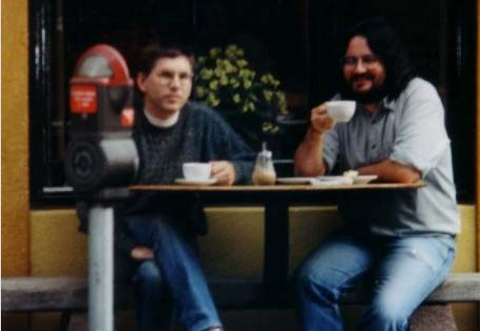
\includegraphics[width=0.5\textwidth]{../Part1/figure/RossAndRobert}
  \newline
  R was created by Ross Ihaka and Robert Gentleman as an open source alternative to S. First release in 1993.
\end{frame}

\begin{frame}{Nearly 40 years of development}
  \begin{figure}%
      \centering
      \subfloat{{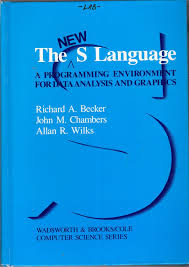
\includegraphics[width=0.27\textwidth]{../Part1/figure/NewSlanguage} }}%
      \qquad
      \subfloat{{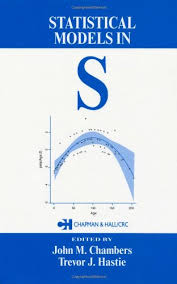
\includegraphics[width=0.27\textwidth]{../Part1/figure/StatisticalModelsinS} }}%
      \qquad
      \subfloat{{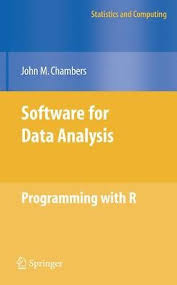
\includegraphics[width=0.27\textwidth]{../Part1/figure/Soda} }}
      \label{fig:example}%
  \end{figure}
\end{frame}

\begin{frame}{R package growth}
  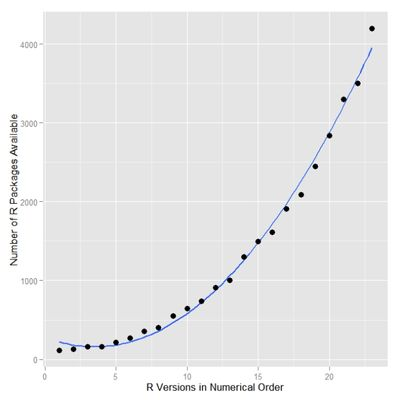
\includegraphics[height=0.75\textheight]{../Part1/figure/rPackages}
\end{frame}

\begin{frame}
Several packages developed for actuarial use:
  \begin{itemize}
    \item actuar
    \item ChainLadder
    \item lossDev
    \item favir
    \item MRMR
  \end{itemize}
\end{frame}

\begin{frame}{Books about R for actuaries!}
  \begin{figure}%
      \centering
      \subfloat{{
\includegraphics[width=0.27\textwidth]{../Part1/figure/ComputationalActuarialScience} }}%
      \qquad
      \subfloat{{
\includegraphics[width=0.27\textwidth]{../Part1/figure/PredictiveModeling} }}%
      \qquad
      \subfloat{{
\includegraphics[width=0.27\textwidth]{../Part1/figure/RegressionModeling} }}
      \label{fig:example}%
  \end{figure}
\end{frame}

\begin{frame}{What's RStudio?}
RStudio is an Integrated Development Environment (IDE). It's not necessary, but provides quite a few nice features:
  \begin{itemize}
    \item Edit multiple scripts at a time, syntax coloring
    \item Manage projects, version control
    \item View variables in memory, debug code
    \item Support for package development
    \item Reproducible research
  \end{itemize}
\end{frame}

\begin{frame}
Does R and RStudio work for everyone?
\end{frame}

\begin{frame}[fragile]{Basics}
  \begin{itemize}
    \item Basic command entry
    \item How to get help
    \item Working directory
    \item Console vs. script
  \end{itemize}
\end{frame}

\begin{frame}[fragile]
\begin{knitrout}\tiny
\definecolor{shadecolor}{rgb}{0.969, 0.969, 0.969}\color{fgcolor}\begin{kframe}
\begin{alltt}
\hlnum{1} \hlopt{+} \hlnum{1}
\end{alltt}
\begin{verbatim}
## [1] 2
\end{verbatim}
\begin{alltt}
\hlstd{r} \hlkwb{=} \hlnum{4}
\hlnum{2} \hlopt{*} \hlstd{pi} \hlopt{*} \hlstd{r}\hlopt{^}\hlnum{2}
\end{alltt}
\begin{verbatim}
## [1] 100.5
\end{verbatim}
\end{kframe}
\end{knitrout}

\begin{knitrout}\tiny
\definecolor{shadecolor}{rgb}{0.969, 0.969, 0.969}\color{fgcolor}\begin{kframe}
\begin{verbatim}
## ?plot
## ??cluster
\end{verbatim}
\end{kframe}
\end{knitrout}

\begin{knitrout}\tiny
\definecolor{shadecolor}{rgb}{0.969, 0.969, 0.969}\color{fgcolor}\begin{kframe}
\begin{alltt}
\hlkwd{getwd}\hlstd{()}
\end{alltt}
\begin{verbatim}
## [1] "C:/Users/bfannin/R/Projects/RPM2014/Part1"
\end{verbatim}
\end{kframe}
\end{knitrout}

\begin{knitrout}\tiny
\definecolor{shadecolor}{rgb}{0.969, 0.969, 0.969}\color{fgcolor}\begin{kframe}
\begin{alltt}
\hlkwd{setwd}\hlstd{(}\hlstr{"~/SomeNewDirectory/SomeSubfolder"}\hlstd{)}

\hlcom{# Save your script}

\hlkwd{source}\hlstd{(}\hlstr{"SomefileName.R"}\hlstd{)}
\end{alltt}
\end{kframe}
\end{knitrout}

\end{frame}

\begin{frame}
%Pause
\begin{itemize}
  \item Can everyone type in basic commands?
  \item Can everyone create, open, save and source a script?
  \item Has everyone set their working directory to the location of the data files we'll use?
\end{itemize}
\end{frame}

\begin{frame}[fragile]{Reading data}
\begin{knitrout}
\definecolor{shadecolor}{rgb}{0.969, 0.969, 0.969}\color{fgcolor}\begin{kframe}
\begin{alltt}
\hlstd{myData} \hlkwb{=} \hlkwd{read.csv}\hlstd{(}\hlstr{"SomeFile.csv"}\hlstd{)}
\end{alltt}
\end{kframe}
\end{knitrout}

\end{frame}

\begin{frame}[fragile]{Reading from Excel}
\begin{knitrout}
\definecolor{shadecolor}{rgb}{0.969, 0.969, 0.969}\color{fgcolor}\begin{kframe}
\begin{alltt}
\hlkwd{library}\hlstd{(XLConnect)}
\hlstd{wbk} \hlkwb{=} \hlkwd{loadWorkbook}\hlstd{(}\hlstr{"myWorkbook.xlsx"}\hlstd{)}
\hlstd{df} \hlkwb{=} \hlkwd{readWorksheet}\hlstd{(wbk, someSheet)}
\end{alltt}
\end{kframe}
\end{knitrout}

\end{frame}

\begin{frame}[fragile]{Reading from the web - 1}
\begin{knitrout}\tiny
\definecolor{shadecolor}{rgb}{0.969, 0.969, 0.969}\color{fgcolor}\begin{kframe}
\begin{alltt}
\hlstd{URL} \hlkwb{=} \hlstr{"http://www.casact.org/research/reserve_data/ppauto_pos.csv"}
\hlstd{df} \hlkwb{=} \hlkwd{read.csv}\hlstd{(URL,} \hlkwc{stringsAsFactors} \hlstd{=} \hlnum{FALSE}\hlstd{)}
\end{alltt}
\end{kframe}
\end{knitrout}

\end{frame}

\begin{frame}[fragile]{Reading from the web - 2}
\begin{knitrout}\tiny
\definecolor{shadecolor}{rgb}{0.969, 0.969, 0.969}\color{fgcolor}\begin{kframe}
\begin{alltt}
\hlkwd{require}\hlstd{(XML)}
\hlstd{URL} \hlkwb{=} \hlstr{"http://www.pro-football-reference.com/teams/nyj/2012_games.htm"}
\hlstd{games} \hlkwb{=} \hlkwd{readHTMLTable}\hlstd{(URL,} \hlkwc{stringsAsFactors} \hlstd{=} \hlnum{FALSE}\hlstd{)}
\end{alltt}
\end{kframe}
\end{knitrout}

\end{frame}

\begin{frame}[fragile]{Reading from a database}
\begin{knitrout}
\definecolor{shadecolor}{rgb}{0.969, 0.969, 0.969}\color{fgcolor}\begin{kframe}
\begin{alltt}
\hlkwd{library}\hlstd{(RODBC)}
\hlstd{myChannel} \hlkwb{=} \hlkwd{odbcConnect}\hlstd{(}\hlkwc{dsn} \hlstd{=} \hlstr{"MyDSN_Name"}\hlstd{)}
\hlstd{df} \hlkwb{=} \hlkwd{sqlQuery}\hlstd{(myChannel,} \hlstr{"SELECT stuff FROM myTable"}\hlstd{)}
\end{alltt}
\end{kframe}
\end{knitrout}

\end{frame}

\begin{frame}[fragile]{Data frames}
Every time we read in data, we're creating a data frame. The data frame is a seminal concept in R. Most statistical operations expect one and they are the most common way to pass data in and out of R.

Although critical to understand, this is very, very easy to get. What's a data frame? It's a table. That's it.
\begin{knitrout}
\definecolor{shadecolor}{rgb}{0.969, 0.969, 0.969}\color{fgcolor}\begin{kframe}
\begin{alltt}
\hlstd{df} \hlkwb{=} \hlkwd{read.csv}\hlstd{(}\hlstr{"SomeFile.csv"}\hlstd{)}
\hlkwd{View}\hlstd{(df)}
\end{alltt}
\end{kframe}
\end{knitrout}

\end{frame}

\begin{frame}[fragile]{A simple script}
\begin{knitrout}
\definecolor{shadecolor}{rgb}{0.969, 0.969, 0.969}\color{fgcolor}\begin{kframe}
\begin{alltt}
\hlstd{N} \hlkwb{=} \hlnum{100}
\hlstd{B0} \hlkwb{=} \hlnum{5}
\hlstd{B1} \hlkwb{=} \hlnum{1.5}

\hlkwd{set.seed}\hlstd{(}\hlnum{1234}\hlstd{)}

\hlstd{e} \hlkwb{=} \hlkwd{rnorm}\hlstd{(N,} \hlkwc{mean} \hlstd{=} \hlnum{0}\hlstd{,} \hlkwc{sd} \hlstd{=} \hlnum{1}\hlstd{)}
\hlstd{X1} \hlkwb{=} \hlkwd{rep}\hlstd{(}\hlkwd{seq}\hlstd{(}\hlnum{1}\hlstd{,} \hlnum{10}\hlstd{),} \hlnum{10}\hlstd{)}

\hlstd{Y} \hlkwb{=} \hlstd{B0} \hlopt{+} \hlstd{B1} \hlopt{*} \hlstd{X1} \hlopt{+} \hlstd{e}

\hlstd{df} \hlkwb{=} \hlkwd{data.frame}\hlstd{(Y, X1, e)}
\hlstd{myFit} \hlkwb{=} \hlkwd{lm}\hlstd{(Y} \hlopt{~} \hlstd{X1,} \hlkwc{data} \hlstd{= df)}
\end{alltt}
\end{kframe}
\end{knitrout}

\end{frame}

\begin{frame}[fragile]{So what have we done?}
\begin{knitrout}
\definecolor{shadecolor}{rgb}{0.969, 0.969, 0.969}\color{fgcolor}\begin{kframe}
\begin{alltt}
\hlstd{N} \hlkwb{=} \hlnum{100}

\hlstd{B0} \hlkwb{=} \hlnum{5}

\hlstd{B1} \hlkwb{=} \hlnum{1.5}
\end{alltt}
\end{kframe}
\end{knitrout}

Assign a number to a variable (i.e. enter a value into a single cell in a spreadsheet).
\end{frame}

\begin{frame}[fragile]
\begin{knitrout}
\definecolor{shadecolor}{rgb}{0.969, 0.969, 0.969}\color{fgcolor}\begin{kframe}
\begin{alltt}
\hlkwd{set.seed}\hlstd{(}\hlnum{1234}\hlstd{)}
\end{alltt}
\end{kframe}
\end{knitrout}

Set the seed for random number generation.
\end{frame}

\begin{frame}[fragile]
\begin{knitrout}
\definecolor{shadecolor}{rgb}{0.969, 0.969, 0.969}\color{fgcolor}\begin{kframe}
\begin{alltt}
\hlstd{e} \hlkwb{=} \hlkwd{rnorm}\hlstd{(N,} \hlkwc{mean} \hlstd{=} \hlnum{0}\hlstd{,} \hlkwc{sd} \hlstd{=} \hlnum{1}\hlstd{)}
\hlstd{X1} \hlkwb{=} \hlkwd{rep}\hlstd{(}\hlkwd{seq}\hlstd{(}\hlnum{1}\hlstd{,} \hlnum{10}\hlstd{),} \hlnum{10}\hlstd{)}
\end{alltt}
\end{kframe}
\end{knitrout}


Every variable is a vector. Think of a set of cells in a spreadsheet. Here, e is a vector with N values. X1 is the sequence of integers from 1 through 10 repeated 10 times. Vectors can grow and shrink automatically. No need to move cells around on a sheet. No need to copy formulas or change named ranges.
\end{frame}

\begin{frame}[fragile]
Vectorization is one of the most important concepts in R!

Similar to Matlab/Octave, operations on a table in a database.
\begin{knitrout}
\definecolor{shadecolor}{rgb}{0.969, 0.969, 0.969}\color{fgcolor}\begin{kframe}
\begin{alltt}
\hlstd{Y} \hlkwb{=} \hlstd{B0} \hlopt{+} \hlstd{B1} \hlopt{*} \hlstd{X1} \hlopt{+} \hlstd{e}
\end{alltt}
\end{kframe}
\end{knitrout}

Vectors may be used in arithmetic operations. Y is now a vector with length equal to the longest vector used in the calculation.

Question: B0 and B1 are vectors of length 1. X1 and e are vectors of length 100. How are they combined?
\end{frame}

\begin{frame}[fragile]{Recycling}
R will "recycle" vectors until there are enough rows to perform an operation, i.e. everything gets as "long" as the longest vector in the operation. For scalar operations on a vector this doesn't involve any drama. Try the following code:
\begin{knitrout}\tiny
\definecolor{shadecolor}{rgb}{0.969, 0.969, 0.969}\color{fgcolor}\begin{kframe}
\begin{alltt}
\hlstd{vector1} \hlkwb{=} \hlnum{1}\hlopt{:}\hlnum{10}
\hlstd{vector2} \hlkwb{=} \hlnum{1}\hlopt{:}\hlnum{5}
\hlstd{scalar} \hlkwb{=} \hlnum{3}

\hlkwd{print}\hlstd{(vector1} \hlopt{+} \hlstd{scalar)}
\end{alltt}
\begin{verbatim}
##  [1]  4  5  6  7  8  9 10 11 12 13
\end{verbatim}
\begin{alltt}
\hlkwd{print}\hlstd{(vector2} \hlopt{+} \hlstd{scalar)}
\end{alltt}
\begin{verbatim}
## [1] 4 5 6 7 8
\end{verbatim}
\begin{alltt}
\hlkwd{print}\hlstd{(vector1} \hlopt{+} \hlstd{vector2)}
\end{alltt}
\begin{verbatim}
##  [1]  2  4  6  8 10  7  9 11 13 15
\end{verbatim}
\end{kframe}
\end{knitrout}

\end{frame}

\begin{frame}[fragile]{Fit a linear model}
\begin{knitrout}
\definecolor{shadecolor}{rgb}{0.969, 0.969, 0.969}\color{fgcolor}\begin{kframe}
\begin{alltt}
\hlstd{myFit} \hlkwb{=} \hlkwd{lm}\hlstd{(Y} \hlopt{~} \hlstd{X1)}
\end{alltt}
\end{kframe}
\end{knitrout}

We've just created a linear model where Y depends on X1. We don't need to specify the length of the response or the design matrix. Later, we'll see how R will automatically create a complicated design matrix automatically.
\end{frame}

\begin{frame}[fragile]
\begin{knitrout}\tiny
\definecolor{shadecolor}{rgb}{0.969, 0.969, 0.969}\color{fgcolor}\begin{kframe}
\begin{alltt}
\hlkwd{summary}\hlstd{(myFit)}
\end{alltt}
\begin{verbatim}
## 
## Call:
## lm(formula = Y ~ X1, data = df)
## 
## Residuals:
##    Min     1Q Median     3Q    Max 
## -2.188 -0.742 -0.228  0.629  2.709 
## 
## Coefficients:
##             Estimate Std. Error t value Pr(>|t|)    
## (Intercept)   4.8383     0.2181    22.2   <2e-16 ***
## X1            1.5009     0.0351    42.7   <2e-16 ***
## ---
## Signif. codes:  0 '***' 0.001 '**' 0.01 '*' 0.05 '.' 0.1 ' ' 1
## 
## Residual standard error: 1.01 on 98 degrees of freedom
## Multiple R-squared:  0.949,	Adjusted R-squared:  0.948 
## F-statistic: 1.82e+03 on 1 and 98 DF,  p-value: <2e-16
\end{verbatim}
\end{kframe}
\end{knitrout}

\end{frame}

\begin{frame}{Installing packages}
Several ways: 
\begin{enumerate}
  \item From a CRAN mirror
  \item Locally
  \item Copy someone else's library directory
  \item From GitHub
\end{enumerate}
The library path may be anywhere! If you have a local document repository
this is a great place to store packages without irritating your IT dept.
\end{frame}

\begin{frame}[fragile]
\begin{knitrout}
\definecolor{shadecolor}{rgb}{0.969, 0.969, 0.969}\color{fgcolor}\begin{kframe}
\begin{alltt}
\hlkwd{.libPaths}\hlstd{()}
\hlstd{packageDir} \hlkwb{=} \hlkwd{.libPaths}\hlstd{()[}\hlnum{1}\hlstd{]}
\hlkwd{list.files}\hlstd{(packageDir)}

\hlkwd{install.packages}\hlstd{(}\hlstr{"ggplot2"}\hlstd{)}

\hlkwd{remove.packages}\hlstd{(}\hlstr{"IdontWantThisAnymore"}\hlstd{)}

\hlcom{# Load an installed package into memory}
\hlkwd{library}\hlstd{(MRMR)}

\hlcom{# Will load the package and return TRUE/FALSE}

\hlcom{# if the package could be loaded}
\hlkwd{require}\hlstd{(MRMR)}
\end{alltt}
\end{kframe}
\end{knitrout}

\end{frame}

\begin{frame}
%Pause
Can everyone install a package?
\end{frame}
\end{document}
